\documentclass[10pt]{beamer}

\usetheme{TUMHaas}

\usepackage{textpos}
\usepackage{upgreek}
\usepackage{slashed}
\usepackage{rotating}

\setlength{\TPHorizModule}{1mm}
\setlength{\TPVertModule}{1mm}
\setlength{\fboxrule}{10pt}

\setbeamercovered{transparent}
\setbeamertemplate{navigation symbols}{}

% define colours
\definecolor{TUMblue}{HTML}{0065bd}
\definecolor{tum_pantone540}{HTML}{00335B}

\DeclareGraphicsExtensions{.pdf,.png,.jpg}
\newcommand<>{\highlighton}[1]{
  \alt#2{\structure{#1}}{{#1}}
}

\newcommand{\icon}[1]{\pgfimage[height=1em]{#1}}

%***********************************Title*********************************


\graphicspath{{logos/},{grafix/}}

\pdfinfo
{
  /Title       (Dark Matter Reinterpretation using Razor Variable and Simplified Models)
%  /Creator     
  /Author      (Lingxin Meng)
}


\title[Dark Matter Reinterpretation]{Dark Matter Reinterpretation\\using Razor Variables and Simplified Models}

\author[Lingxin Meng (lingxin.meng@cern.ch)]{Lingxin Meng}


\institute[]{}

%\date{{May 15, 2014}
\date{{\today}\\
\vspace{1cm}

	}

\titlegraphic{
%	
\includegraphics[height=0.6cm]{logo_tum}\hspace{0.3cm}
%	
\includegraphics[height=1cm]{e18_logo_croped}\hspace{0.3cm}
%	
\includegraphics[height=1cm]{ClusterLogo_ohne}\hspace{0.3cm}
%	
\includegraphics[height=1cm ]{v1_1_black}
%  
\includegraphics[height=0.6cm]{BMBF.pdf}\hspace{0.3cm}

}

%****************************Begin of Document***************************
\begin{document}


%***************table of contents, can be modified
\frame[plain]{\titlepage}

%\section*{}
%\begin{frame}
%  \frametitle{Dark Matter}
%  \tableofcontents[hidesubsections]

%\end{frame}

%\AtBeginSection[]
%{
%  \frame<handout:0>
%  {
%    \frametitle{Outline}
%    \tableofcontents[currentsection,currentsubsections]
%  }
%}

%\AtBeginSubsection[]
%{
%  \frame<handout:0>
% {
%  \frametitle{Outline}
% \tableofcontents[sectionstyle=show/hide,subsectionstyle=show/shaded/hide]
%}
%}




%********************REAL CONTENT****************************************

\section{Dark Matter}
\begin{frame}
\frametitle{What is Dark Matter}
\small
\begin{itemize}
	\item Evidence: astrophysics
	\begin{itemize}
		\item Rotating speed of galaxy spirals
		\item Thickness of galaxy discs
		\item Anisotropies in CMB
		\item Gravitational lensing of Bullet Cluster
	\end{itemize}
	\item Criteria
	\begin{itemize}
		\item Lifetime
		\item No electromagnetic interaction
		\item Relic mass density
	\end{itemize}
	\item Candidates
	\begin{itemize}
		\item Primordial black holes
		\item Axions
		\item Sterile neutrinos
		\item \textbf{WIMPs}
	\end{itemize}
\end{itemize}
\begin{minipage}[c]{0.58\textwidth}

\end{minipage}
\begin{minipage}[c]{0.4\textwidth}
	\vspace{1.5mm}
\end{minipage}

\end{frame}

\begin{frame}
\small
\frametitle{WIMPs}
\begin{itemize}
	\item Weakly Interacting Massive Particles (10\,GeV -- 10\,TeV)
	\item Produced in the early Universe's "freeze-out"
	\item Relic density with self-annihilation cross-section $\widehat{=}$ weak scale
	%$\langle \upsigma \upnu \rangle \simeq 3\times10^{-26}\,\text{cm}^3\text{s}^{-1}$ 
	\item MSSM prediction: weakly interacting particle with 100\,GeV\\
	$\rightarrow$ ``WIMP miracle''
\end{itemize}

\end{frame}

\begin{frame}
\frametitle{Why LHC?}
\small

\begin{minipage}[c][][c]{0.69\textwidth}
DM detection:
\begin{itemize}
	\item Direct Search: nuclear recoil spectrum
	\begin{itemize}
		\item Low recoil energy
		\item Backgrounds
		\item Local DM density
	\end{itemize}
	\item Indirect Search: annihilation \& decay products
	\begin{itemize}
		\item CR background
		\item DM halo density variation
	\end{itemize}
	\item \textbf{Collider}
	\begin{itemize}
		\item Independent from astrophysical assumptions
		\item Complementary to direct and indirect searches
		\item If couple to g or q, DM could be produced
		\item Signature: missing transverse energy
	\end{itemize}
\end{itemize}
\end{minipage}
\begin{minipage}[c][0.9\textheight][b]{0.25\textwidth}
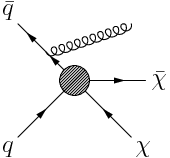
\includegraphics[width=1\textwidth]{dm_lhc}
\end{minipage}
\end{frame}

\begin{frame}
\frametitle{Object and Constraints}
\small
\begin{block}{\small Missing Energy}
{
\begin{minipage}[c][][c]{0.59\textwidth}
\begin{itemize}
	\item ATLAS: nearly 4$\uppi$
	\item No SM charge $\rightarrow$ escape
	\item Jet reconstruction
	\item $\slashed{E}_\text{T} = E_{\text{tot}} - E_{\text{rec}}$
\end{itemize}
\end{minipage}
\begin{minipage}[c][][c]{0.4\textwidth}
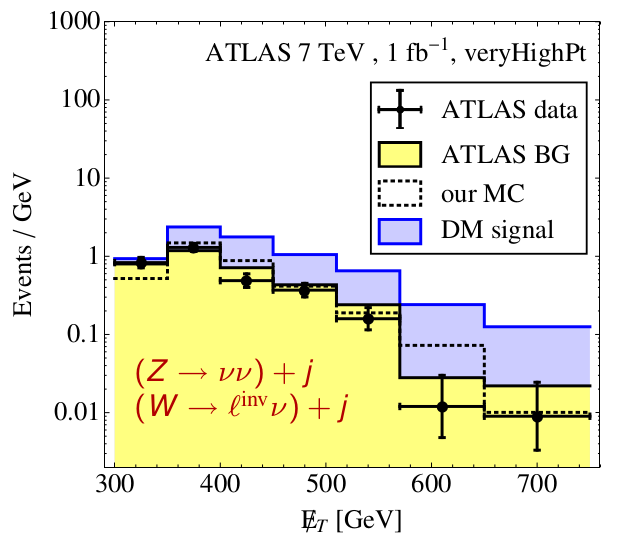
\includegraphics[width=1\textwidth]{met_spectrum}
\end{minipage}
}
\end{block}

\begin{block}{\small Effective Field Theory vs. Simplified Models}
{

\begin{minipage}[t][][t]{0.49\textwidth}
\begin{itemize}
	\item Momentum transfer in order of direct \& indirect searches
	\item Contact interaction
\end{itemize}
\end{minipage}
\begin{minipage}[t][][t]{0.49\textwidth}
\begin{itemize}
	\item Momentum transfer $> M_{\text{Med}}$
	\item Underlying interactions	
\end{itemize}
\end{minipage}
}
\end{block}

\end{frame}


\section{My Contribution}
\begin{frame}
\frametitle{Razor Analysis}
\small
\begin{itemize}
	\item Razor analysis on simplified models and EFT
	\item Discriminate heavy pair productions from SM backgrounds
	\item No assumption on $\slashed{E}_\text{T}$
	\item Backgrounds follow clean exponential distributions
	\item Two reconstructed objects in the final state\\
	$\rightarrow$ ``megajets'', equal and opposite in the beam direction
	\item ``Hemisphere''-algorithm
	\item Complementary dataset to monojet search
\end{itemize}

\hrulefill

\begin{minipage}[c][][c]{0.49\textwidth}
Razor variables:
	\begin{align*}
		M_\text{R} & = \sqrt{(E_{\text{j}_1}+E_{\text{j}_2})^2 - (p^{\text{j}_1}_\text{z} + p^{\text{j}_2}_\text{z})^2} \\
		M^\text{T}_\text{R} & = \sqrt{\slashed{E}_\text{T} (p^{\text{j}_1}_\text{T} + p^{\text{j}_2}_\text{T}) - \vec{\slashed{E}}_\text{T} \cdot (\vec{p}^{\text{j}_1}_\text{T} + \vec{p}^{\text{j}_2}_\text{T})} \\
		R & = \frac{M^\text{T}_\text{R}}{M_\text{R}}
	\end{align*}
\end{minipage}\hfill
\begin{minipage}[c][][c]{0.49\textwidth}
	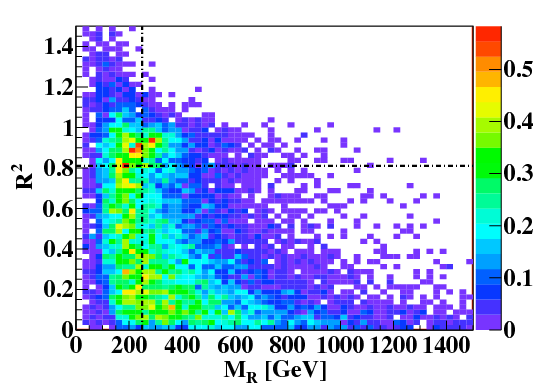
\includegraphics[width=0.9\textwidth]{razor_dm.png}
\end{minipage}

\end{frame}

\begin{frame}
\frametitle{Event Selection}

\begin{itemize}
%	for monojet
%	\item Monojet: one unbalanced high $\text{p_T}$ jet \rightarrow large $\text{E^{miss}_T}$
	\item Trigger on $\slashed{E}_\text{T} > $ 40\,GeV
	\item Primary vertex and $>$ 5 tracks
%	\item Highest $p_\text{T}$ jet
%	\item No e or $\upmu$
%	\item Non-collision background: requirements on $p_\text{T} >$ 20\,GeV and $\mid \eta \mid >$ 4.5
	
%	for razor
%	\item MLM matching of 60\,GeV
	\item Jets: $p_\text{T} >$ 60\,GeV, $\mid \eta \mid < $ 3.0
	\item e ($\upmu$): $p_\text{T} > $ 20(10)\,GeV, $\mid \eta \mid < $ 2.5(2.1)
	\item Include hadronically decaying $\uptau$ that suffice jet definition
	\item Signal region: leading jet with high $p_\text{T}$ and high $\slashed{E}_\text{T}$
\end{itemize}

\end{frame}

\begin{frame}
\frametitle{Tools}
\begin{itemize}
	\item MadGraph 5 - event generator
	\item Pythia 8 - parton shower
	\item AToM - Automated Testing of Models
	\begin{itemize}
		\item PGS - detector smearing
		\item Rivet - analysis \& histograms
	\end{itemize}

\end{itemize}
\end{frame}

\begin{frame}
\frametitle{Plan}
\begin{itemize}
	\item Collaboration with other summer students
	\item Write a monojet analysis 
	\begin{itemize}
		\item Use both EFT and simplified models for modelling of DM
		\item Compare the limits
	\end{itemize}
	\item Check the impact of the Razor analysis on signal selection
\end{itemize}
\end{frame}

%\begin{frame}[noframenumbering]
%\frametitle{Backup Slide}
%\framesubtitle{Meh}
%\end{frame}

\end{document}
